\documentclass{article}

% if you need to pass options to natbib, use, e.g.:
% \PassOptionsToPackage{numbers, compress}{natbib}
% before loading nips_2016
%
% to avoid loading the natbib package, add option nonatbib:
% \usepackage[nonatbib]{nips_2016}

%\usepackage[final]{nips_2016}

% to compile a camera-ready version, add the [final] option, e.g.:
\usepackage[final]{nips_2016}

\usepackage[utf8]{inputenc} % allow utf-8 input
\usepackage[T1]{fontenc}    % use 8-bit T1 fonts
\usepackage{hyperref}       % hyperlinks
\usepackage{url}            % simple URL typesetting
\usepackage{booktabs}       % professional-quality tables
\usepackage{amsfonts}       % blackboard math symbols
\usepackage{nicefrac}       % compact symbols for 1/2, etc.
\usepackage{microtype}      % microtypography
\usepackage{amsmath}
\usepackage{amssymb}
\usepackage{graphicx}

\title{Deep Q-Learning with Recurrent Neural Networks}

% The \author macro works with any number of authors. There are two
% commands used to separate the names and addresses of multiple
% authors: \And and \AND.
%
% Using \And between authors leaves it to LaTeX to determine where to
% break the lines. Using \AND forces a line break at that point. So,
% if LaTeX puts 3 of 4 authors names on the first line, and the last
% on the second line, try using \AND instead of \And before the third
% author name.

\author{
  Clare Chen \\
  \texttt{cchen9@stanford.edu} \\
  \And
  Vincent Ying \\
  \texttt{vincenthying@stanford.edu} \\
  \And
  Dillon Laird \\
  \texttt{dalaird@cs.stanford.edu} \\
}

% Remove NIPS footer
\pagestyle{empty}

\begin{document}
% \nipsfinalcopy is no longer used

\maketitle

\begin{abstract}
  Deep reinforcement learning models have proven to be successful at learning
  control policies image inputs. They have, however, struggled with learning
  policies that require longer term information. Recurrent neural network
  architectures have be used in tasks dealing with longer term dependencies
  between data points. We investigate these architectures to overcome the
  difficulties arising from learning policies with long term dependencies.
\end{abstract}

\section{Introduction}
    Recent advances in Reinforcement Learning have led to human-level or greater
    performance on a wide variety of games (e.g. Atari 2600 Games).  However,
    training these networks can take a long time, and the techniques presented in
    the state of the art [add reference] perform poorly on several games that
    require long term planning.  Deep Q-Networks learn to estimate the Q-Values
    (long term discounted returns) of selecting each possible action from the
    current game state. \\
    \\
    Deep Q-networks are limited in the sense that they learn a mapping from a
    limited number of past states, or game screens.  In practice, DQN is trained
    using an input consisting of the last four states (or game screens).  Thus,
    DQN performs poorly at games that require the agent to remember information
    more than four screens ago.  In other words, the game could no longer be
    modeled as a true Markov Decision Process; all of the information needed to
    make an optimal action would no longer be contained in a single state.  We
    explore the concept of a Deep Recurrent Q-network, a combination of a Long
    Short Term Memory (LSTM) [add reference] and a Deep Q-network.  We wish to
    demonstrate that introducing recurrent network architecture into the Deep
    Q-network, the network can retain information from previous frames of the
    game and achieve good performance on games that require long term planning. \\
    \\
    In addition, recent achievements of visual attention models have introduced
    people to exploring the possibility of incorporating attention mechanisms
    into the structure of the DRQN algorithm.  The advantage of using attention
    mechanisms is that DRQN acquires the ability to select and focus on small
    informative regions of an input image, thus helping to reduce the total
    number of parameters in the deep neural network and computation operations
    needed for training and testing.  \\
    \\
    \\
    Deep Q-Networks (DQNs) have had success playing Atari 2600 games [0] but have 
    struggled with particular games involving policies that require longer term
    information. This is evident from the types of games that DQNs perform poorly at,
    near or below human-level, which includes Q*bert, Ms. Pac-Man, and in an extreme
    case Montezuma's Revenge.

    \begin{figure}[h]
        \centering
        \begin{minipage}{0.8\textwidth}
            \centering
            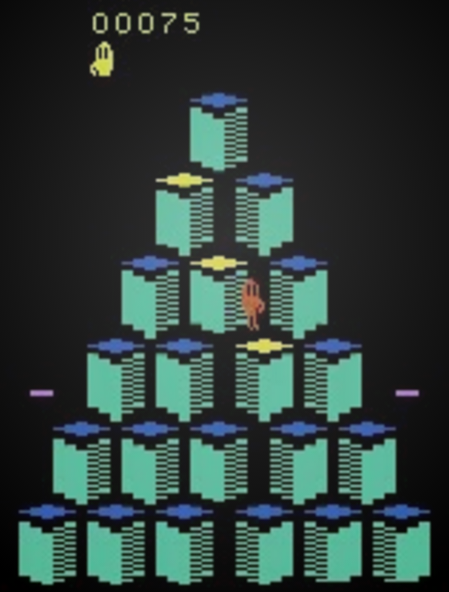
\includegraphics[scale=0.15]{Qbert}
            \centering
            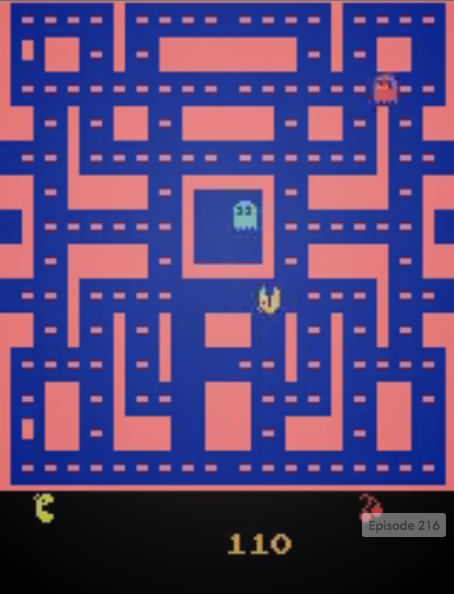
\includegraphics[scale=0.15]{MsPacman}
            \centering
            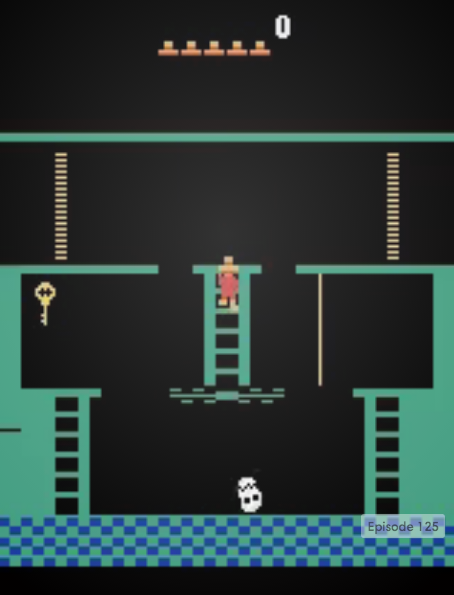
\includegraphics[scale=0.15]{MontezumaRevenge}
        \end{minipage}
        \caption{Q*bert, Ms. Pac-Man and Montezuma's Revenge}
    \end{figure}
    
    Recurrent neural networks (RNNs) have been used in modeling longer sequences and
    is one way to overcome DQNs difficulties with learning policies that require longer
    term information. We investigate augmenting DQN architecture proposed in [0], utilizing
    a convolutional neural network (CNN), with an RNN.

\section{Recurrent Deep Q-Learning}
We propose two architectures for the Recurrent Deep Q-Network (RDQN). The first
is a very basic extension of DQN. We look at the last $L$ states, $\{s_{t-(L-1)},
\dots, s_{t}\}$ and feed these into a convolutional neural network (CNN) to get
intermediate outputs $\text{CNN}(s_{t-i}) = x_{t-i}$. These are then fed into a
RNN, $\text{RNN}(x_{t-i}) = h_{t-i}$, and the final output $h_t$ is used to
predict the $Q$ value.

\begin{figure}[h]
    \centering
    \includegraphics[scale=0.5]{RDQN}
    \caption{Architecutre of the RDQN}
\end{figure}

Another architecture we used was a version of an attention RNN. For the attention
RNN we take the $L$ hidden states outputted by the RNN, $\{h_{t-(L-1)}, \dots, h_{t}\}$
and we take the inner product with a learned vector $v_a$, $\{v_a^Th_{t-(L-1)}, \dots,
v_a^Th_{t}\}$. We then take a softmax over these values, $a_{t-i} =
\text{softmax}(v_a^Th_{t-i})$. We use this softmax to take a weighted sum over
the hidden states to get a context vector, $c_t = \sum_{i=0}^{L-1}a_{t-i}h_{t-i}$.
This context vector is then used to predict the $Q$ value.

\section{Experiments}
Experiments.

\section*{References}
\small
% TODO: need to figure out how to cite this stuff properly..
[0] "Human-level control through deep reinforcement learning" Volodymyr Mnih, Koray Kavukcuoglu, David Silver, Andrei A. Rusu, Joel Veness, Marc G. Bellemare, Alex Graves, Martin Riedmiller, Andreas K. Fidjeland, Georg Ostrovski, Stig Petersen, Charles Beattie, Amir Sadik, Ioannis Antonoglou, Helen King, Dharshan Kumaran, Daan Wierstra, Shane Legg \& Demis Hassabis \\

[1] "Playing Atari with Deep Reinforcement Learning" Volodymyr Mnih, Koray Kavukcuoglu, David Silver, Alex Graves, Ioannis Antonoglou, Daan Wierstra, Martin Riedmiller \\

[2] "Neural Machine Translation By Jointly Learning To Align and Translate" Dzmitry Bahdanau, Kyunghyun Cho, Yoshua Bengio \\

[3] "Deep Recurrent Q-Learning for Partially Observable MDPs" Matthew Hausknecht and Peter Stone \\

[4] "Prioritized Experience Replay" Tom Schaul, John Quan, Ioannis Antonoglou, and David Silver \\

[5] "Effective Approaches to Attention-based Neural Machine Translation" Minh-Thang Luong, Hieu Pham, and Christopher D. Manning \\

[6] "Neural Machine Translation By Jointly Learning To Align And Translate" Dzmitry Bahdanau, KyungHyun Cho, and Yoshua Bengio \\

[7] "Deep Attention Recurrent Q-Network" Ivan Sorokin, Alexey Seleznev, Mikhail Pavlov, Aleksandr Fedorov, and Anastasiia Ignateva \\



\end{document}
